\documentclass[12pt]{article}

\usepackage[margin=1in]{geometry}
\usepackage{fancyhdr}
\pagestyle{fancy}
\usepackage{amsmath}
\usepackage{amssymb}

% limit to particular location
\usepackage{float}

% graphics
\usepackage{graphicx}
% for subfigures
\usepackage{subcaption}

% better ref links
\usepackage{hyperref}

% footnote in footer
\newcommand{\fancyfootnotetext}[2]{%
  \fancypagestyle{dingens}{%
    \fancyfoot[LO,RE]{\parbox{7cm}{\footnotemark[#1]\footnotesize #2}}%
  }%
  \thispagestyle{dingens}%
}

\lhead{HW3}
\chead{Digital Image Processing}
\rhead{B03902036}


\begin{document}

\section*{Problem 1}
\subsection*{Boundary extraction}
\begin{figure}[H]
    \centering
    \begin{subfigure}[t]{0.24\textwidth}
        \centering
        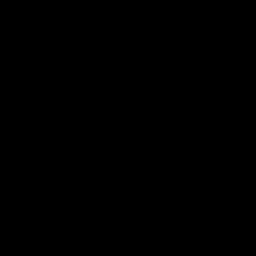
\includegraphics[height=1.5in]{images/B_m1}
        \caption{$1 \times 1$}
    \end{subfigure}%
    ~ 
    \begin{subfigure}[t]{0.24\textwidth}
        \centering
        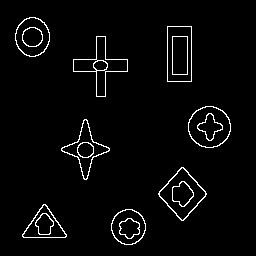
\includegraphics[height=1.5in]{images/B_m3}
        \caption{$3 \times 3$}
    \end{subfigure}%
    ~
    \begin{subfigure}[t]{0.24\textwidth}
        \centering
        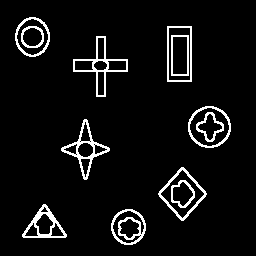
\includegraphics[height=1.5in]{images/B_m5}
        \caption{$5 \times 5$}
    \end{subfigure}%
    ~
    \begin{subfigure}[t]{0.24\textwidth}
        \centering
        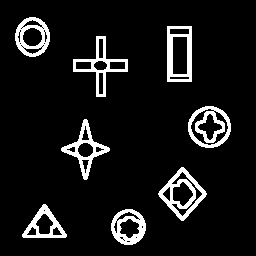
\includegraphics[height=1.5in]{images/B_m7}
        \caption{$7 \times 7$}
    \end{subfigure}
    \caption{$B$}
\end{figure}
Boundary extraction is composed of erosion and its complement
\begin{equation}
	B = I_1 \wedge \sim (I_1 \ominus SE)
\end{equation}
where $SE$ is the structural element, square in this case.
When the sides of $SE$ increases, the more the erosion is applied on $I_1$, causing more blanked region appeared after $\& ~(I_1 \ominus SE)$, leading to thicker edges.

\subsection*{Counting objects}
The algorithm is described below 
\begin{enumerate}
\item 
Pick a non-zero pixel by scanning sequentially from the origin. Name this one pixel image as $A$. 

\item
Start from that location, dilate $A$ using structure element $SE$, a 3-by-3 square in this case.
Dilate until $A$ stops expansion, in comparison to the input image $I_1$.

\item 
Set the selected pixels in $A$ as value of $N$, a book-keeping variable, and increment $N$.

\item
Remove selected pixels in $A$ from $I_1$.

\item
Repeat this process until $I_1$ is empty.
\end{enumerate}
Though there is the possibility to modify size and shape of $SE$, since we are interesting in selecting the object, with $SE$ being too wide will certainly cause the algorithm to miss it or accidentally select its neighbor. Therefore, 3 is kept here.

\begin{figure}[H]
    \centering
    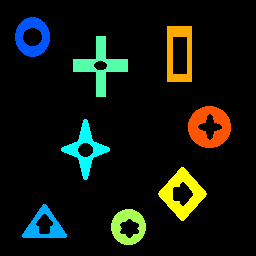
\includegraphics[height=2.5in]{images/L}
    \caption{Labeled connected components}
\end{figure}

One may consider using running length encoding to efficiently sort the result, since RLE can better utilize the cache mechanism, but two-pass is still required similar to the naive implementation provided here.

During writing of the erosion algorithm, I also found out the slide misplaced result of Sternberg and Serra definition, despite the equations themselves are correct.

\subsection*{Skeletonizing}
\begin{figure}[H]
    \centering
    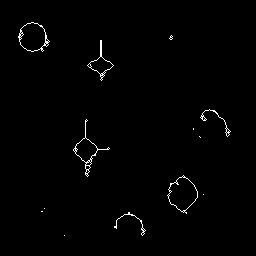
\includegraphics[height=2.5in]{images/S}
    \caption{$S$, skeletonized $I_1$}
\end{figure}
The implementation try to follow the implementation from textbook, which requires two set of lookup tables. General operation is 
\begin{equation}
	G = X \cap \lbrack \sim M \cup P \rbrack
\end{equation}
where $X$ is the input image, $G$ is the output image, $M$ is the conditional marker determined in the process, and $P$ is the inhibiting variable.

During the first pass, $M$ is determined by hit-and-miss transformation using the kernel from \autoref{tbl:conditional}. 
I put tons of time to figure out the decimal equivalent of them, I might as well put my result here, and there seems to be no one posting this out there on the Net.
\begin{table}[H]
\caption{Conditional}
	\centering
	\begin{tabular}{c|c}	
	Type & Decimal number \\
	\hline
	\hline
	S1 & 64, 16, 4, 1\\
	S2 & 128, 32, 8, 2\\
	S3 & 192, 96, 48, 24, 12, 6, 3, 129 \\
	TK4 & 160, 40, 10, 130 \\
	STK4 & 193, 112, 28, 7 \\
	ST5 & 176, 161, 104, 194, 224, 56, 14 ,131 \\
	ST6 & 177, 108 \\
	STK6 & 240, 225, 120, 60, 15, 135, 195 \\
	STK7 & 241, 124, 31, 199\\
	STK8 & 227, 248, 62, 143\\
	STK9 & 243, 231, 252, 249, 124, 63, 159, 207\\
	STK10 & 247, 253, 127, 223\\
	K11 & 251, 254, 191, 239\\
	\end{tabular}
	\label{tbl:conditional}
\end{table}

During the second pass, which is coined as the unconditional stage, output result is determined by combination of $X$ and $M$. 
Since there are spaces for combinations in the textbook kernel list, I separated them to three categories to ease the computation process.

\paragraph{First} type is simply equal-or-not comparison with values from \autoref{tbl:unconditional_eq}. One simply extract the surrounding pixels 
\begin{equation}
	V = \sum_{i\in\text{neighbors}}{M_i 2^i}
\end{equation}
where $V$ is the corresponding decimal value constructed by the fully connected neighbors.
Most significant bit is the first pixel, designated $M_0$ in the textbook.

\begin{table}[H]
\caption{Unconditional, EQ}
	\centering
	\begin{tabular}{c|c}	
	Type & Decimal number \\
	\hline
	\hline
	Spur & 1, 4, 64, 16\\
	4-connected & 2, 128, 8, 32\\
	L & 160, 40, 130, 10
	\end{tabular}
	\label{tbl:unconditional_eq}
\end{table}

\paragraph{Second} type requires one to provide a mask before comparison.
The comparison is composed of two parts
\begin{equation}
\begin{cases}
	P_1 = (X \vee K_M) \wedge K_C \\
	P_2 = (T \wedge \sim K_M) \wedge (K_C \wedge \sim K_M)\\
\end{cases}
\label{eq:unconditional_or_eq_eq}
\end{equation}
and the final result is determined by 
\begin{equation}
	P = P_1 \wedge P_2
\end{equation}
$P_1$ used the mask to ignore flexible $D$ terms in the table provided in the textbook, while $P_2$ verifies the constant terms, $M$, $0$ and $1$ are satisfied as well.
$K_M$ is the mask while $K_C$ is the conditional equivalent decimal number, both of them are enlisted as a pair $(K_M, K_C)$ in \autoref{tbl:unconditional_or_eq}.

\begin{table}[H]
\caption{Unconditional, OR-EQ}
	\centering
	\begin{tabular}{c|c}	
	Type & (Mask, Condition) \\
	\hline
	\hline
	Corner & (31, 255), (241, 255), (199, 255), (124, 255) \\
	Tee & (84, 252), (213, 255), (117, 255), (93, 255) \\
	Diagonal & (17, 181), (68, 109), (17, 91), (68, 214)\\
	\end{tabular}
	\label{tbl:unconditional_or_eq}
\end{table}

\paragraph{Third} type is similar to the second type, but instead of equivalent, it requires unequal, since in the textbook, 
\begin{equation}
	A \cup B \cup C = 1
\end{equation}
in other words, one of them has to be 1, complementary is relatively easy to test for.

Under this consensus, \autoref{eq:unconditional_or_eq_eq} can be modified as
\begin{equation}
\begin{cases}
	P_1 = \sim ((X \vee K_M) \vee K_C) \\
	P_2 = (T \wedge \sim K_M) \wedge (K_C \wedge \sim K_M)\\
\end{cases}
\label{eq:unconditional_or_eq_eq}
\end{equation}

\begin{table}[H]
\caption{Unconditional, OR-NEQ}
	\centering
	\begin{tabular}{c|c}	
	Type & (Mask, Condition) \\
	\hline
	\hline
	Vee & (184, 248), (42, 62), (138, 143), (162, 227) \\
	\end{tabular}
\end{table}

If short segments are unwanted, pruning algorithm can be employed. In my implementation, some objects seem to being thinned too aggressively, however, I haven't found the pitfalls in the pipeline for the time being. 

\section*{Problem 2}
\subsection*{Law's method}
\begin{figure}[H]
    \centering
    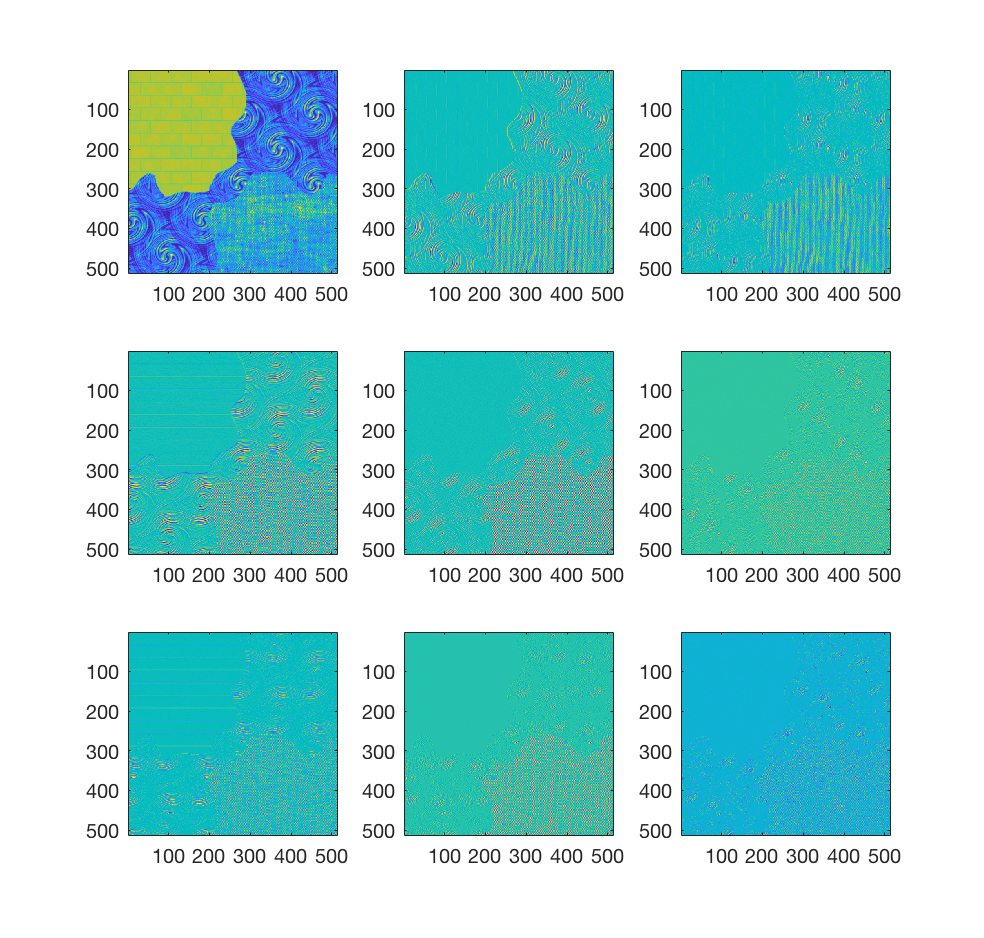
\includegraphics[height=5in]{images/M}
    \caption{Filters}
    \label{fig:law_filters}
\end{figure}
\autoref{fig:law_filters} shows the results after applying 3-by-3 filters described in the slides, oriented from left-to-right, top-to-bottom are low-to-high pass.

The result is not quite clear in this case, however, the simple energy function of windows size 15,
\begin{equation}
	T = \cap \cap_{(i, j) \in w} M(i, j)^2
\end{equation}
yields fabulous result.

\begin{figure}[H]
    \centering
    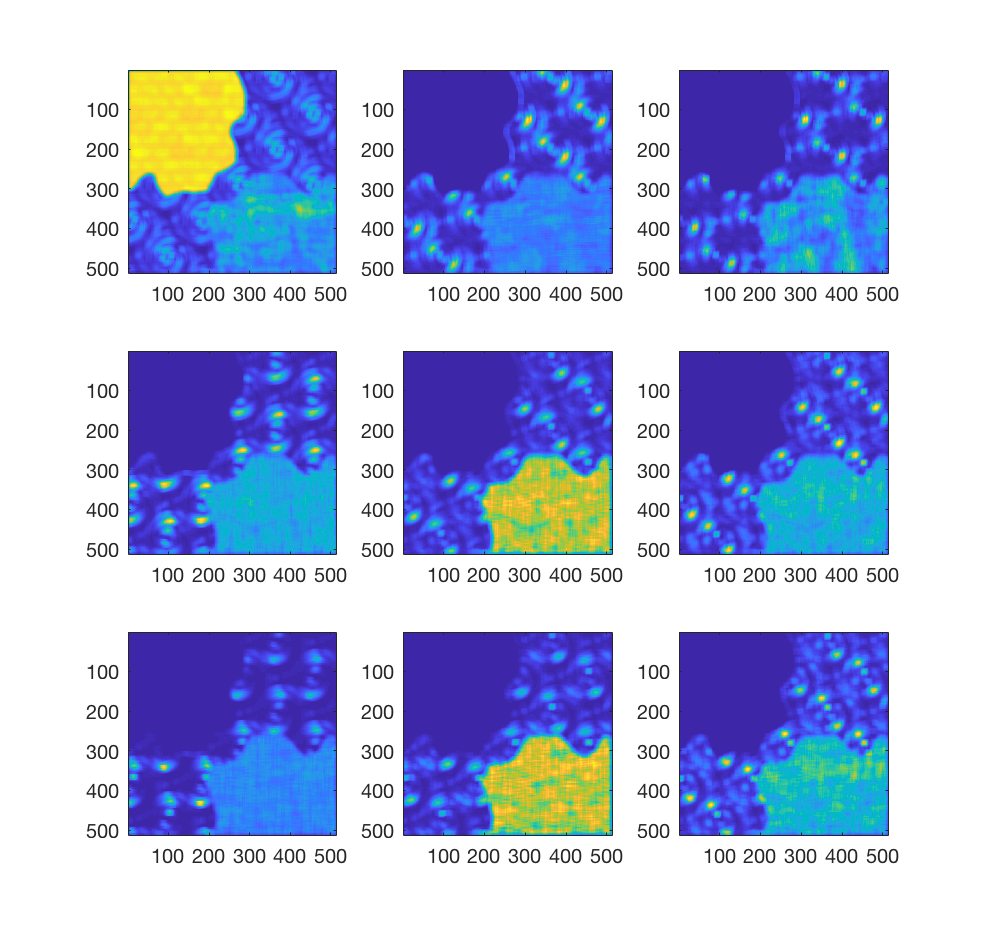
\includegraphics[height=5in]{images/T}
    \caption{Energy}
    \label{fig:law_energy}
\end{figure}
\autoref{fig:law_energy} oriented the same way as \autoref{fig:law_filters}, in this case, we can easily see the whirls have their frequency components evenly distributed, while the cloth on the lower right is relatively high frequency, compares to the brick wall on the upper left side.

Using classic K-mean clustering algorithm with three classes and randomly initialized seeds, results in acceptable result.

\begin{figure}[H]
    \centering
    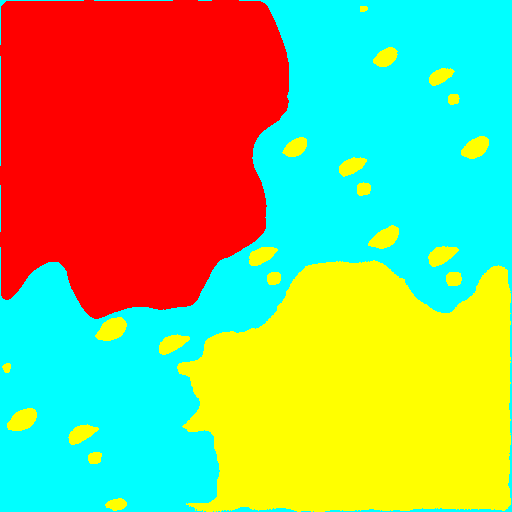
\includegraphics[height=2.5in]{images/K}
    \caption{Segmented reuslt}
    \label{fig:kmean}
\end{figure}

However, blobs can be observed in the middle section of the whirls, one may remove them by removing objects smaller then specified size.

\subsection*{Texture swapping}
Efos-Leung algorithm is adapted for this task, courtesy to the MATLAB implementation presented by {\it asteroidhouse} on GitHub, with small modification, one can adapt the algorithm for partial texture synthesis (patch the regions, relatively smaller), instead of full synthesis (generate entire image from a small patch). 

The algorithm generates the texture pixel-wise, outwards from the initial seed, using pixels inside a defined windows as the context. 
The basic idea is modeling the patch as a generalized Markov chain, similar to the $n$-gram idea in natural language processing. 
Therefore, one build a probability for tables for each $n$-gram pixel combinations through repeatedly sample in the window, and synthesize new pixels by observing the most probable intensity in the sampled $n$-gram "corpus".

\begin{figure}[H]
    \centering
    \begin{subfigure}[t]{0.3\textwidth}
        \centering
        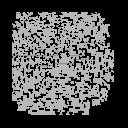
\includegraphics[height=2in]{images/tex1}
        \caption{Class 1}
        \label{fig:synth_1}
    \end{subfigure}%
    ~ 
    \begin{subfigure}[t]{0.3\textwidth}
        \centering
        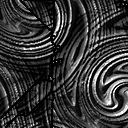
\includegraphics[height=2in]{images/tex2}
        \caption{Class 2}
        \label{fig:synth_2}
    \end{subfigure}%
    ~
    \begin{subfigure}[t]{0.3\textwidth}
        \centering
        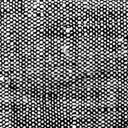
\includegraphics[height=2in]{images/tex3}
        \caption{Class 3}
        \label{fig:synth_3}
    \end{subfigure}%
    \caption{Synthesized}
    \label{fig:synth}
\end{figure}

Using random patch size pick in the regions, no larger than 128-by-128, due to deadline, window size is configured to 4, and synthesis result size is restricted to 128-by-128 instead of full size 512-by-512. 
\autoref{fig:synth} shows the synthesized result of three identified categories retrieved from previous section.
Synthesis iteration is limited to 1000 due to limited time as well, instead of ensuring all the pixels are determined.

As one may expected, insufficient window size will result in information lost, causing the texture unable to be continuous, visualized as the crack in \autoref{fig:synth_2}.
The brick pattern requires much larger window to capture the grid lines, this will significantly increase the synthesis time, very limited window and limited iteration cycle not only lead to incomplete output, but also incorrect pattern in \autoref{fig:synth_1}. 

For pattern that has high frequency components, visualized in \autoref{fig:law_energy}, relatively small window and less iteration is required as hypothesized, the result in \autoref{fig:synth_3} is pleasing as well.


Unable to generate complete synthesized swapped image on time.

\end{document}
              